\documentclass[onecolumn]{article}
\usepackage{graphicx,color,psfrag}
\usepackage[caption=false,font=footnotesize]{subfig}
\usepackage{amsmath,amssymb}
\usepackage{cite}
\usepackage[]{subfig} % subfloats
\usepackage{verbatim}
\usepackage{listings}
\usepackage{upquote} % Make copy/paste of single quotes work properly % use \char"0D inside text
\usepackage{enumitem}  % single-spaced enumerations
%\setlist[enumerate]{itemsep=0mm} % single-spaced enumerations

\usepackage{booktabs}
%\usepackage[title,titletoc,toc]{appendix}

\usepackage[multidot]{grffile} % allow dots in graphics filenames
\usepackage[usenames,dvipsnames]{xcolor}
\definecolor{DarkGreen}{rgb}{0,0.35,0.1}
\usepackage[pagebackref=true, breaklinks=true, colorlinks=true, bookmarks=true, citecolor=DarkGreen, linkcolor=DarkGreen, urlcolor=DarkGreen]{hyperref}
\usepackage{url}
\usepackage{breakurl}
\usepackage{fancyvrb}
\usepackage[nowarn]{glossaries}
\glsdisablehyper % no hyperlinks for glossary entries
\usepackage{siunitx} % for non-italics mu in units

\setcounter{section}{-1} % quick start gets a section number 0

%---default figure placement
\makeatletter
  \providecommand*\setfloatlocations[2]{\@namedef{fps@#1}{#2}}
\makeatother
\setfloatlocations{figure}{bt}
\setfloatlocations{table}{bt}
%---

\title{
LFCamExplore: Plenoptic Camera Design Explorer\\
{\large v0.1.0 in development }}

\author{Copyright (c) 2017 by Donald G. Dansereau}

\date{\today}

\makeglossaries % touch then rm .glo file in build to use rubber
% Regular usage managed by 'glossaries'
%
% | Shortcut |    Default   | Description
% +----------+--------------+---------------------------------------------------
% |   \ac    |    \gls      | entry
% |   \Ac    |    \Gls      | entry, capitalised
% |   \acp   |    \glspl    | plural form of the entry
% |   \Acp   |    \Glspl    | plural form of the entry, capitalised
%
%
% To force 'glossaries' to use a particular element of the acronym definition:
%
% | Shortcut |    Default   | Description
% +----------+--------------+---------------------------------------------------
% |   \acs   |  \acrshort   | acronym
% |   \Acs   |  \Acrshort   | acronym, capitalised
% |   \acsp  |  \acrshortpl | plural acronym
% |   \Acsp  |  \Acrshortpl | plural acronym for the entry, capitalised
% |   \acl   |  \acrlong    | description
% |   \Acl   |  \Acrlong    | description, capitalised
% |   \aclp  |  \acrlongpl  | plural description
% |   \Aclp  |  \Acrlongpl  | plural description, capitalised
% |   \acf   |  \acrfull    | description and acronym
% |   \Acf   |  \Acrfull    | description and acronym, capitalised
% |   \acfp  |  \acrfullpl  | description and acronym plural
% |   \Acfp  |  \Acrfullpl  | description and acronym plural, capitalised
%
%
% To reset all acronyms call:
%
%    \glsresetall
%
% NOTES:
%  - it is preferable to capitalise only proper nouns in the definitions
%  - to enable the shortcut commands, 'glossaries' must be instantiated using
%    \usepackage[shortcuts]{glossaries}


\newacronym{AUV}{AUV}{autonomous underwater vehicle}
\newacronym{UAV}{UAV}{unmanned aerial vehicle}
\newacronym{USV}{USV}{unmanned surface vehicle}
\newacronym{UGV}{UGV}{unmanned ground vehicle}
\newacronym{GPS}{GPS}{global positioning system}
\newacronym{SLAM}{SLAM}{simultaneous localization and mapping}

\newacronym{MDSP}{MDSP}{multi-dimensional signal processing}
\newacronym{ROS}{ROS}{region of support}
%\newacronym{DOF}{DOF}{degree-of-freedom}
\newacronym{RMS}{RMS}{root mean square}
\newacronym{SNR}{SNR}{signal-to-noise ratio}
\newacronym{CNR}{CNR}{contrast-to-noise ratio}
\newacronym{PCA}{PCA}{principal component analysis}

\newacronym{FIR}{FIR}{finite impulse response}
\newacronym{IIR}{IIR}{infinite impulse response}
\newacronym{DFT}{DFT}{discrete Fourier transform}
\newacronym{FFT}{FFT}{fast Fourier transform}
\newacronym{PSNR}{PSNR}{peak signal-to-noise ratio}
\newacronym{FPGA}{FPGA}{field programmable gate array}
\newacronym{GPU}{GPU}{graphics processing unit}
\newacronym{ASIC}{ASIC}{application-specific integrated circuit}
\newacronym{BW}{BW}{bandwidth}

\newacronym{PSF}{PSF}{point spread function}
\newacronym{OTF}{OTF}{optical transfer function}
\newacronym{MTF}{MTF}{magnitude transfer function}
\newacronym{FOV}{FOV}{field of view}
\newacronym{BRDF}{BRDF}{bidirectional reflectance distribution function}
\newacronym{FWHM}{FWHM}{full width at half maximum}
\newacronym{DOF}{DOF}{depth of field}

\newacronym{RANSAC}{RANSAC}{random sampling and consensus}
 

% stop breaking inline equations across lines
%\relpenalty=9999  
%\binoppenalty=9999
%% window/orphan control
\widowpenalty=10000
\clubpenalty=10000

% Shortcuts for building the function reference
\newcommand{\NewTag}{\protect{~\color{red} \tiny NEW}}
\newcommand{\DeclareFunction}[1]{\hypertarget{#1}{#1}}
\newcommand{\CiteFunction}[1]{\hyperlink{#1}{\small #1}}
\newcommand{\SupFunction}[1]{{\small #1}}

\newcommand{\NewFunctionHeading}[1]{
\hspace{-1.5em}\begin{minipage}[t]{\linewidth}
\noindent\rule{\linewidth}{\arrayrulewidth}
\vspace{0.5em}\hspace{1pt}\textbf{\large #1}\\[-1.1em]
\rule{\linewidth}{\arrayrulewidth}\par\vspace{0.2em}
}

\newcommand{\NewFunctionEntry}[3]{%
\vspace{0.4em}%
	\hspace{1em}\begin{minipage}[t]{\linewidth}%
	\textbf{\DeclareFunction{#1}#2}%
	\end{minipage}\vspace{0.2em}\par
	\hspace*{3em}\begin{minipage}[t]{0.9\linewidth}%
	\protect #3 \vspace{0.4em}
	\end{minipage}%
	\par%
}

\newcommand{\EndFunctionHeading}{
\end{minipage}\vspace{1em}\par
}

% Shortcuts for creating an annotated folder structure
\newcommand{\NewAnnotatedTree}[1]{\vspace{1em}\noindent\begin{tabular}{*{#1}{p{0.1em}}cp{6.5cm}}}
\newcommand{\EndAnnotatedTree}{\end{tabular}\vspace{1em}}
\newcommand{\AnnotatedTreeEntry}[4]{\Repeat{#1}{&}\multicolumn{#2}{l}{\SymbolText{#3}} & \small #4}

\newcommand{\SymbolText}[1]{\texttt{\small #1}}

\RecustomVerbatimEnvironment
{Verbatim}{Verbatim}
{formatcom={\footnotesize}, fontfamily=courier}

\begin{document}

\maketitle
\thispagestyle{empty}\pagestyle{plain}

%-----------------------------
\noindent
Homepage: \url{http://dgd.vision/Tools/LFCamExplore/}

\vspace{1em}\noindent
Requires the Light Field Toolbox for MATLAB v0.4 \url{https://goo.gl/RHe4hR}.

\vspace{1em}\noindent 
Suggestions, bug reports, code improvements and new functionality are solicited -- email \SymbolText{Donald.Dansereau+LFToolbox} \small{at} \SymbolText{gmail} \small{dot} \SymbolText{com}.


\newpage
\tableofcontents
\newpage

%-----------------------------
%-----------------------------
\section{Quick Start}

Install the light field toolbox for MATLAB, restart MATLAB, then run \SymbolText{LFCamExploreGUI.m}.  The windows currently don't auto-arrange, so drag and resize to taste.  The GUI should look like Fig.~\ref{fig_AnnotatedScreenshot}.  Load the provided examples using the ``LOAD'' button, and observe changes in the spatial and sampling pattern displays as you modify the camera design and display settings.

\begin{figure}[h!]
	\centering
	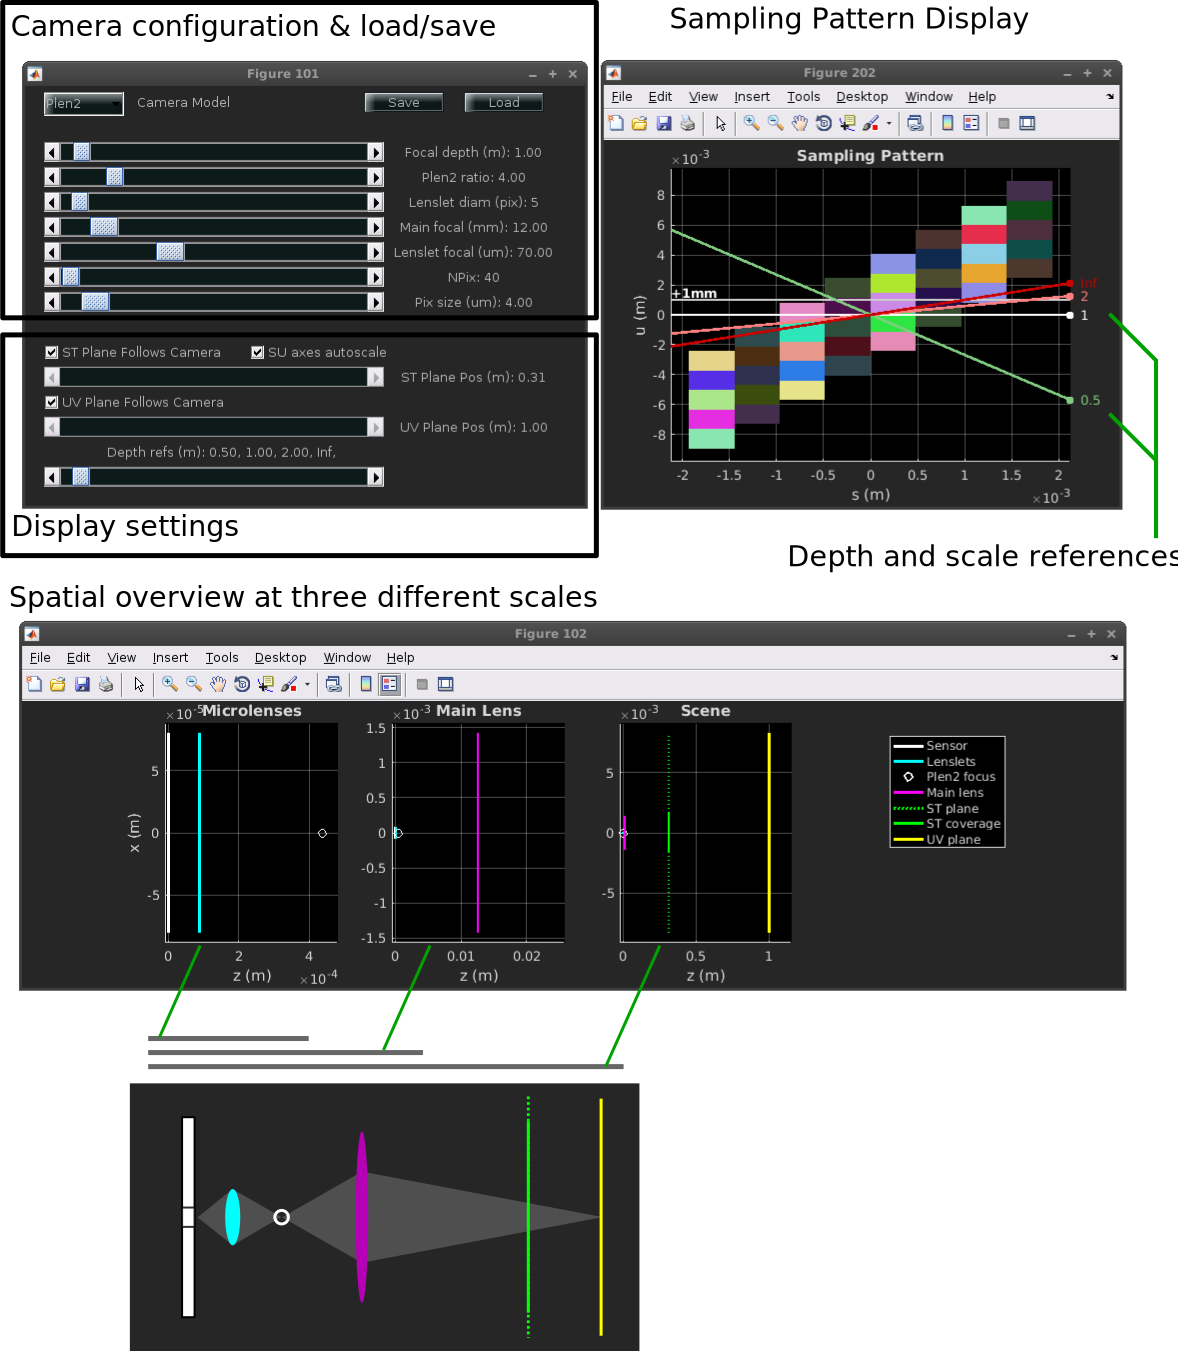
\includegraphics[width=1\textwidth]{Figs/AnnotatedScreenshot}
	\caption{GUI Structure}
	\label{fig_AnnotatedScreenshot}
\end{figure}



%-----------------------------
%-----------------------------
\section{Introduction}

This is a tool for building intuition in the design space of plenoptic cameras.  It can simulate both ``focused'' (aka ``plenoptic 2.0'') cameras as in the design by Lumsdaine and Georgiev, and ``afocal'', ``standard'' or ``plenoptic 1.0'' cameras following Ng's design.

The GUI is broken into three windows, as shown in Fig.~\ref{fig_AnnotatedScreenshot}.  It accepts camera descriptions in terms of lens and sensor properties, and solves for a valid plenoptic camera based on those properties.

The key outputs are a spatial overview of the physical layout of the camera, and a display depicting the sampling pattern of the camera.

%-----------------------------
\subsection{Intended Audience}

This tool is intended for those wanting to design their own plenoptic cameras.  The behaviours of these cameras are not always obvious, and this tool is designed as an intuition builder around the tradeoffs inherent in this design space.  

For those wanting to learn more, Sect.~\ref{sect_FirstSomeBackground} briefly touches on some of the core concepts in plenoptic imaging, and Sect.~\ref{sect_FurtherReading} points out some good references for getting started and learning more in this space.

%-----------------------------
\subsection{Capabilities and Limitations}

The core functionality of the program is to take a set of user-controlled parameters, solve for the geometry of a physically achievable camera fitting those parameters, and display the sampling pattern for an idealized model of that camera.  An estimate of key camera performance metrics is also produced in the MATLAB terminal.  Depth references are drawn to allow evaluation with respect to typical scene content.

The camera model is idealized and misses several higher-order effects.  However, the program is still useful for building intuition.

The sampling pattern visualization is not responsive for large pixel counts.  The intent is to visualize a small patch of pixels near the center of the sensor, to understand how the sampling pattern is influenced by key design parameters.  Gross performance metrics can be calculated by editing the camera design (.json) file for a larger pixel count and loading using the ``load'' button, to run non-interactively.

These additional limitations apply:
\begin{itemize}
\item The results are entirely in 2D.  Generalization to 4D should be done with care.
\item This is an early release, the solvers need checking.
\item The camera performance metrics can be misleading and need checking.
\item This deals with paraxial ray optics only, diffraction limits and lens aberrations are not considered and will have important consequences.
\item The solver and visualization only work for an integer number of pixels per lenslet.  This ignores the effect of projection through the lenslet array.  Vignetting is not considered.
\item The sliders are somewhat coarse, and so a text entry would be useful; for now use a text editor to edit then load the .json files.
\end{itemize}

%-----------------------------
\subsection{Conventions}

This program uses the absolute two-plane parameterization with the camera pointed along the $z$ axis, as depicted in Fig.~\ref{fig_RayRepWorldSide}.  Reference plane positions and therefore plane separation $D$ are set by the user.  The camera solver always keeps the sensor at $z=0$, and all distances are measured relative to the origin, not the front of the camera --~this means that a camera focused at a depth of 2~m will have its sensor at $z=0 m$, a focal plane at $z=2 m$, and the distance from the front of the main lens to the scene will be less than 2~m.


%-----------------------------
%-----------------------------
\section{Understanding Sampling Patterns}
\label{sect_FirstSomeBackground}

\begin{figure}
	\centering
	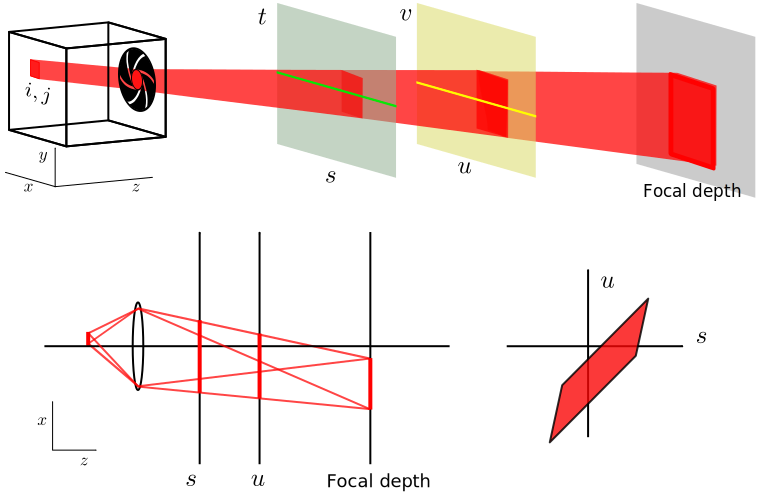
\includegraphics[width=0.85\textwidth]{Figs/Pixel4DParam}
	\caption{Sample pattern for a single pixel in a conventional camera. (top) The camera on the left is focused on the plane to the far right.  The pixel at $i,j$ integrates a subset of the light emanating from the scene, capturing some combinations of position and direction, but not others.  We employ a two-plane parameterization to characterize the rays that the pixel integrates.  (bottom-left) Working in 2D, we see the same situation depicted as a slice in the horizontal plane ($y=0$). (bottom-right) By plotting the points of intersection of each ray with $s$ and $u$, we obtain an epipolar image in $s,u$ for $t,v=0$.  In this space the pixel integrates over a parallelogram.}
	\label{fig_PixelParam2pp}
\end{figure}

\begin{figure}
	\centering
	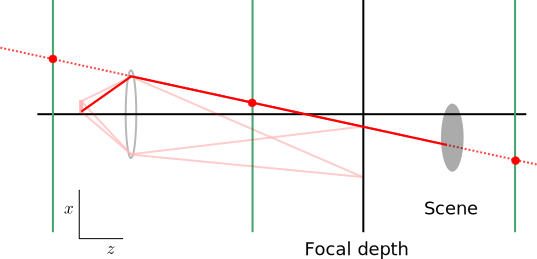
\includegraphics[width=0.85\textwidth]{Figs/RayRepresentation_WorldSide}
	\caption{Rays are finite in extent, but when parameterizing we extend them to infinity.  At the three potential locations for a reference plane shown in green, we see the corresponding points of intersection with the ray as it is extended to infinite length.  We do not deal with the path of the ray after it has been modified by refraction or reflection --~ i.e.~we do not consider its path inside the camera or its intersection with the scene.}
	\label{fig_RayRepWorldSide}
\end{figure}

In this section we review the fundamentals of sampling patterns, epipolar images, and the point-plane correspondence.  Readers familiar with these concepts can skim or skip to Sect.~\ref{sect_SampPatSceneAndCam}.

%-----------------------------
\subsection{Pixels as Integrators of Light}

This tool characterizes a camera's performance in terms of how it samples light in the scene.  All cameras map light to pixels, with each pixel integrating some subset of all the light in the scene --~a subset of the so-called plenoptic function.  Past work has variously characterized the sampling patterns of cameras in terms of how light behaves inside the camera, outside the camera, or a mixture of the two.  Here we choose scene-space characterization in order to allow easy comparison between different camera architectures, and evaluate performance in terms of how the camera measures the world.

Referring to the top of Fig.~\ref{fig_PixelParam2pp}, we assume a camera pointing down the $z$ axis and centered at $x=y=0$, with $y$ pointing up.  We assume the camera is focused at some depth, depicted on the right of the figure, and wish to describe the rays that each of this camera's pixels integrates.  A single pixel at image-space index $i,j$ is shown, and the rays that it integrates are depicted as a red volume.  Note that the camera in this figure is intentionally generic, as the important details are to the right of this figure: which rays did the pixel see?

%-----------------------------
\subsection{Reference Planes}

One can think of a flow of light from the scene towards the camera, with only a small subset of that light eventually reaching any given pixel.  To characterize this subset, we have many choices.  It turns out to be convenient, in the space of plenoptic camera design, to use a light field parameterization in which each ray is described by its point of intersection with each of two reference planes.

By convention we choose the two reference planes as depicted in Fig.~\ref{fig_PixelParam2pp}, an $s,t$ plane and a $u,v$ plane, with each orthogonal to the principal ray of the camera, parallel to each other, and with $s$ and $u$ parallel with $x$, and $t$ and $v$ parallel with $y$.

The positions of the reference planes are arbitrary.  It is important is that the rays being characterized are those emanating from the scene, and not those within the camera.  To accomplish this, rays are treated as lines of infinite extent, even though we know they are generally line segments with finite extent. This is depicted in Fig.~\ref{fig_RayRepWorldSide}. If a reference plane is chosen to be behind the camera relative to the scene, each ray from the scene is extended, as though the camera were not there, until it intersects the plane. Similarly if a reference plane is behind the scene, we extend the rays through the scene until they intersect the reference plane.

We will discuss in Sect.~\ref{sect_RefPlaneLocations} some useful choices for the reference plane positions.

%-----------------------------
\subsection{2D Epipolar Images}

The reference planes give us a 4D description of the rays that each pixel integrates.  This is difficult to visualize in 4D, and so we limit our attention to a horizontal slice of the scene. Referring to the bottom of Fig.~\ref{fig_PixelParam2pp}, we set $y=0$ and consider only each ray's $s$ and $u$ coordinates.  We can plot all those combinations of $s$ and $u$ for which a ray successfully travels from the scene to reach the pixel.  As depicted on the bottom-right of the figure, this results in a surface describing the integrating volume of the pixel~-- in this case, a parallelogram.

A plot depicting the pairs $s,u$ or $t,v$ as in the bottom-right of Fig.~\ref{fig_PixelParam2pp} is called an epipolar plot, and it turns out to be a convenient space in which to understand plenoptic cameras.  From this plot one can visually evaluate complex quantities like depth of field, baseline, and spatial and angular pixel count and resolution.

%-----------------------------
\subsection{How Pixels Appear}

\begin{figure}
	\centering
	\subfloat[]{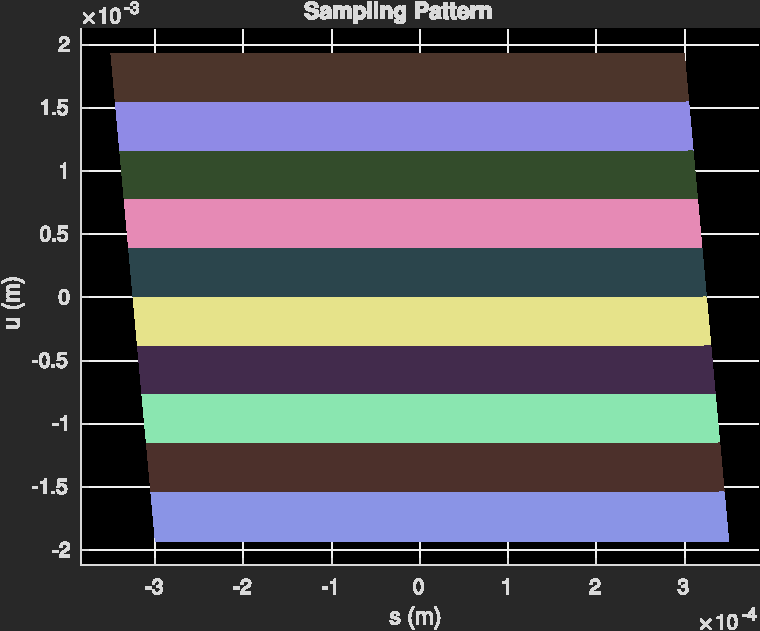
\includegraphics[width=0.3\textwidth]{Figs/SampPatExample_Conventional}\label{subfig_SampPatExampleConventional}} \hfil
	\subfloat[]{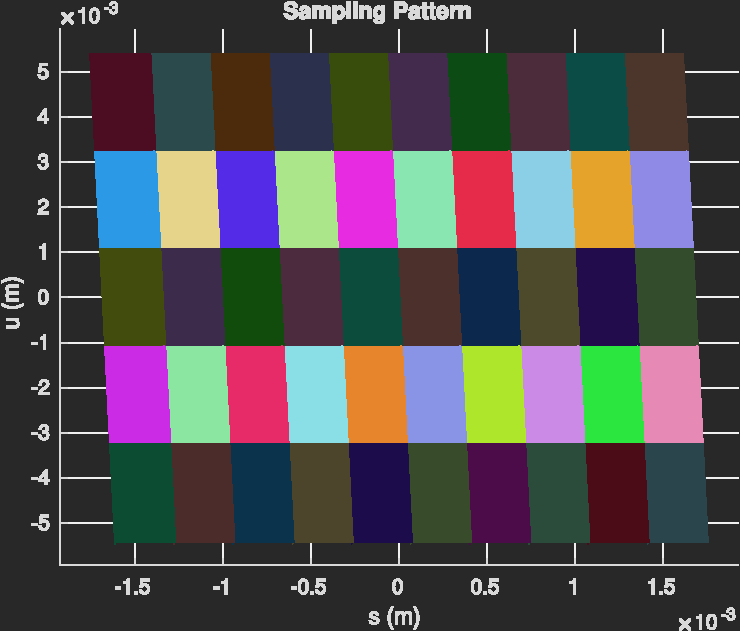
\includegraphics[width=0.3\textwidth]{Figs/SampPatExample_Plen1}\label{subfig_SampPatExamplePlen1}} \hfil
	\subfloat[]{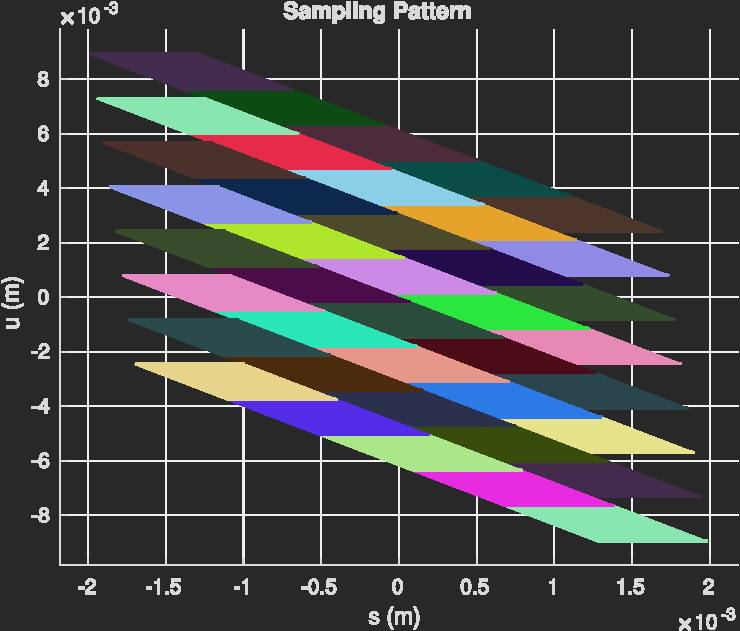
\includegraphics[width=0.3\textwidth]{Figs/SampPatExample_Plen2}\label{subfig_SampPatExamplePlen2}}
	\caption{Example sample patterns for a horizontal group of pixels in (a) a conventional camera, (b) an standard plenoptic camera, and (c) a plenoptic 2.0 camera.}
	\label{fig_SampPatIntro}
\end{figure}

Referring again to Fig.~\ref{fig_PixelParam2pp}, we can see that a single pixel integrates over a parallelogram in the epipolar image.  This is true of both conventional and light field cameras.  The four corners of the parallelogram correspond to the ``marginal'' rays at the edges of the pixel and the aperture.  The four lines depicted in the figure correspond to these four ``marginal'' rays, and to the four corners of the parallelogram in the $s,u$ plot.  For lenslet-based cameras, the four corners are determined by rays at the edges of the pixels and lenslets, and not the edges of the main lens.  This is the phenomenon by which depth of field is decoupled from light gathering in plenoptic cameras.

If we consider multiple pixels in a conventional camera, e.g.~those horizontally adjacent to the first, we can plot each in its own colour to yield an epipolar plot like the one shown in Fig.~\ref{subfig_SampPatExampleConventional}.  For this figure the $s,t$ plane is at the origin, and the $u,v$ plane is at $z = 1$~m, coincident with the focal depth of the camera.  Doing the same for plenoptic cameras in the standard and 2.0 configurations yields tilings of parallelograms in the epipolar image, as seen in Figs.~\ref{subfig_SampPatExamplePlen1} and~\ref{subfig_SampPatExamplePlen2}.  For the standard plenoptic camera, there are 10 pixels per lenslet, appearing horizontally along the figure, and 5 lenslets, appearing vertically.  For the plenoptic 2.0 camera, there are 5 pixels per lenslet and 8 lenslets are depicted.

%-----------------------------
\subsection{How the Scene Appears}

\begin{figure}
	\centering
	\subfloat[]{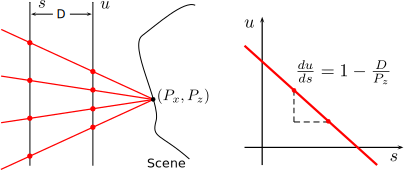
\includegraphics[width=0.6\textwidth]{Figs/PtPlane_su_abs}\label{subfig_PtPlane}}\\
	\subfloat[]{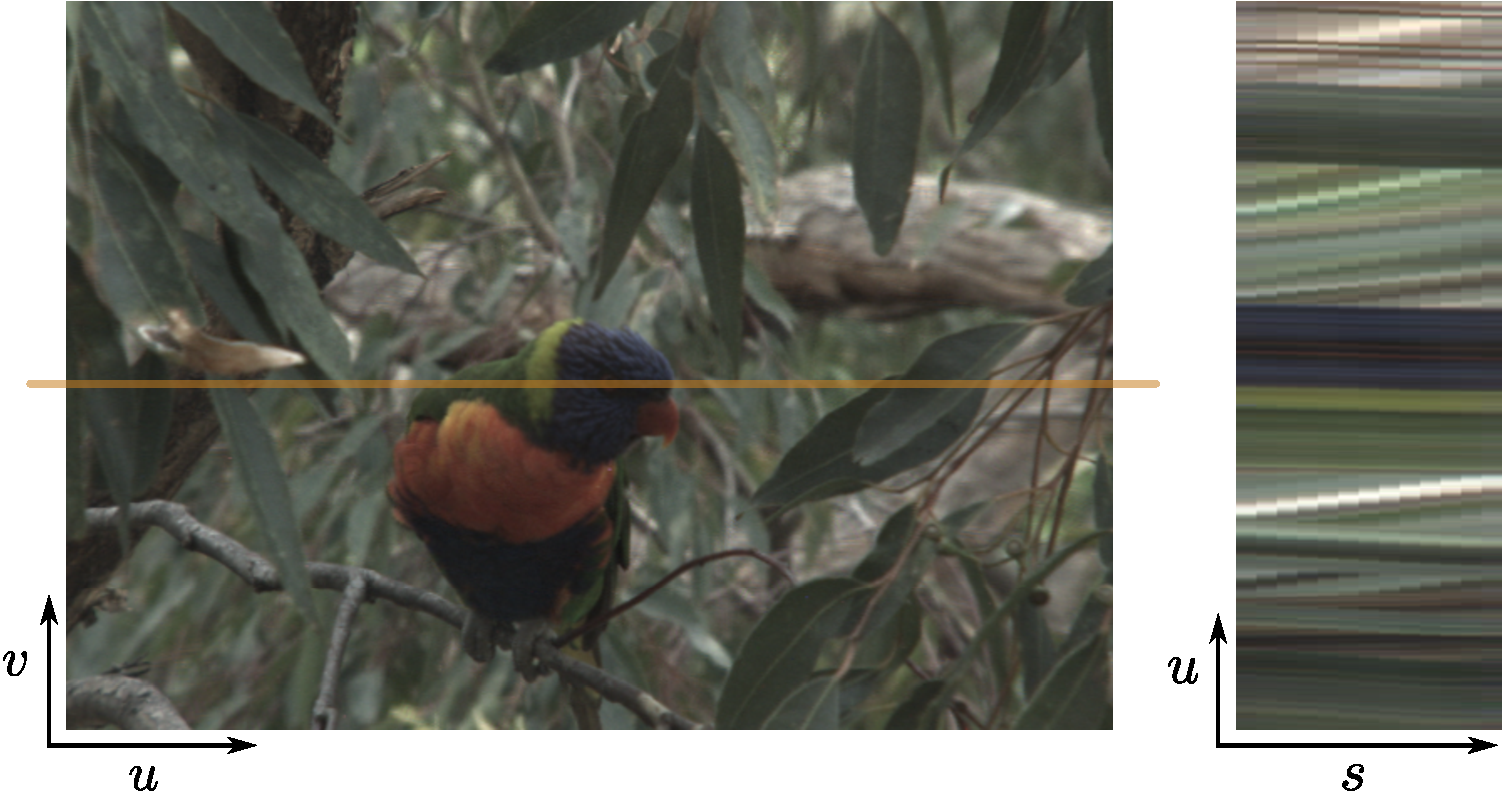
\includegraphics[width=0.8\textwidth]{Figs/SceneExample_SU}\label{subfig_PtPlaneBitmap}}
	\caption{(a, left) A point $P = (P_x,P_y,P_z)$ in the scene emits a pencil of rays which intersect the reference planes following a linear relationship.  (a, right) in the epipolar plane the point appears as a line. The position of the line depends on the 3D position of the point, but its slope is determined entirely by the depth of the point, $P_z$. (b, left) An example scene as a single slice in $u,v$, and (b, right) an epipolar slice taken at the vertical coordinate $v$ marked by the orange line.  Notice objects at different depths appearing at different slopes in the epipolar image.}
	\label{fig_PtPlane}
\end{figure}

So far we've used the epipolar space to describe the rays captured by each pixel of the camera, but this same space can describe the space of rays generated by the scene. Fig.~\ref{subfig_PtPlane} demonstrates the relationship between a point in space and its appearance in the light field.  For rays emanating from a point in space $P = (P_x,P_y,P_z)$, there is a linear relationship between their points of intersection with the $s,t$ and $u,v$ planes.  This linear relationship means the point will appear in an epipolar image as a straight line, with slope related to the depth of the point $P_z$.  This is true regardless of the surface properties at the point.  If the surface happens to be Lambertian, then the line in the epipolar image will be constant-valued.  

By superposition, a set of surfaces in a complex scene will appear as a set of lines in the epipolar image, with parts of the scene at similar depths appearing as lines with similar slopes.  An example of this is shown in Fig.~\ref{subfig_PtPlaneBitmap}.  Taking a horizontal slice of the scene at the bird's eye, we obtain the epipolar image on the right, in which the bird's eye is clearly visible at a slope around $0$

%-----------------------------
\section{The Sampling Pattern Display}
\label{sect_SampPatSceneAndCam}

\begin{figure}
	\centering
	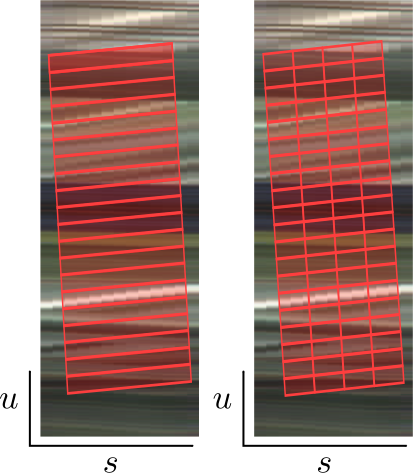
\includegraphics[width=0.4\textwidth]{Figs/SceneAndCamSU}
	\caption{Two examples of the scene's epipolar image overlaid with the camera's sampling pattern: (left) for a conventional camera, and (right) for a plenoptic 1.0 camera. Both cameras are focused on a distant object, corresponding to the bright white streak in the bottom half of the images.}
	\label{fig_SampPatSceneAndCam}
\end{figure}

The performance of a camera for a given scene can be understood by bringing together an epipolar image for the scene, like the one shown in Fig.~\ref{subfig_PtPlaneBitmap}, with the an epipolar image of the sampling pattern, like the ones shown in Fig.~\ref{fig_SampPatIntro}.  Examples of the combined figure are shown in Fig.~\ref{fig_SampPatSceneAndCam}, for cameras focused on a distant object in the scene.  

From this kind of figure we can determine from visual inspection which parts of the scene will appear in focus, which will exhibit defocus blur, based on how textural lines align with the pixels.  The circle of confusion for a point can be evaluated visually.  We can tell which structures will be large enough for the camera to resolve.  The total area of each pixel tells us how much light it receives.  If we were plotting all pixels for the camera, the total extent along $u$ would tell us the camera's \gls{FOV}.  We get an intuition for the camera's ability to distinguish different slopes, and therefore depths in the scene.

The camera design GUI provides exactly this type of figure, but employing depth reference lines to emulate the content of the scene.  


%-----------------------------
\subsection{Depth References}

\begin{figure}
	\centering
	\subfloat[]{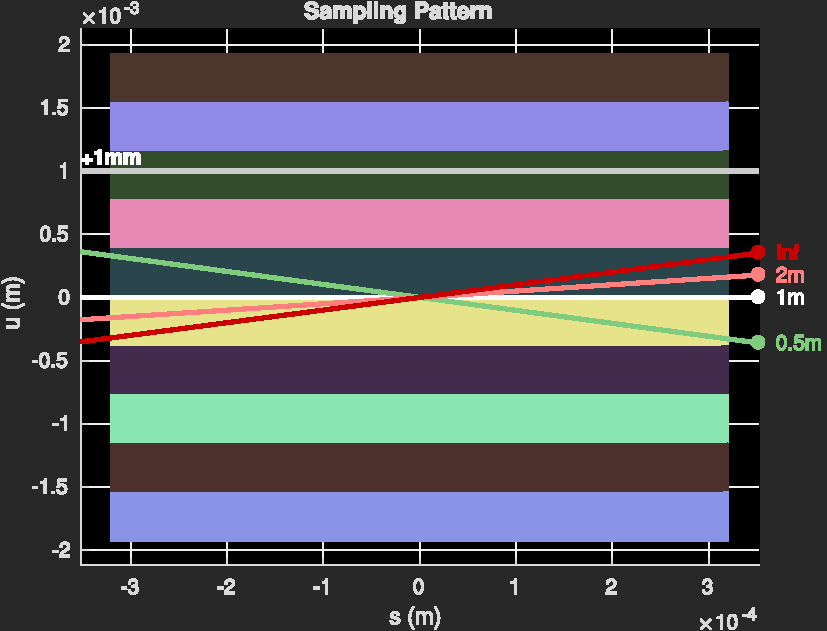
\includegraphics[width=0.48\textwidth]{Figs/SampPatExample_Conventional_WithDepth}\label{subfig_SampPatWithDepthRefConventional}}\hfil
	\subfloat[]{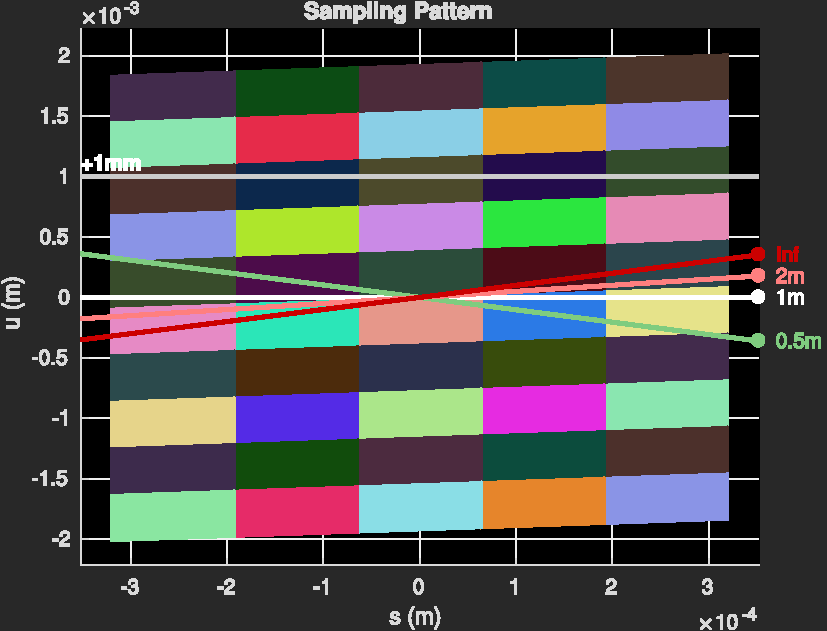
\includegraphics[width=0.48\textwidth]{Figs/SampPatExample_Plen1_WithDepth}\label{subfig_SampPatWithDepthRefPlen1}}
	\caption{(a) Sampling patterns with depth references for (a) a conventional and (b) standard plenoptic camera.}
	\label{fig_SampPatWithDepthRefs}
\end{figure}

In Sect.~\ref{sect_SampPatSceneAndCam} we saw that superimposing the camera's sampling pattern on the scene's epipolar image yields insights into the camera's behaviour.  Rather than displaying a specific scene's epipolar image, the camera design tool displays depth references like those shown in Fig.~\ref{fig_SampPatWithDepthRefs}.  These show the slopes in the epipolar image of scene elements at different depths, allowing visual inspection of the depth of field and textural resolution of the camera.  

The depth references correspond to points lying along the optical axis of the camera, occupying a set of discrete depths.  There is a ``key'' depth reference, shown in white, which is typically chosen to coincide with the focal depth of the camera.  At this key depth, an additional reference is included having a 1~mm offset in the $x$ direction.  This textural reference allows us to evaluate the pixel footprint --~i.e.~the camera's resolution --~at the key depth.  

For example, Fig.~\ref{subfig_SampPatWithDepthRefConventional} depicts a conventional camera.  We can see that the camera is focused at 1~m from the slopes of the pixels compared to the depth references.  A point at 1 or 2~m from the camera will only cross one pixel along $u$ and will therefore appear in focus.  Points at infinity or 0.5~m will cross about 2 pixels, meaning their circle of confusion will be about 2~pixels and they will appear out of focus.  Numerically we confirm that the depth of field of this camera is from about 0.6 to 2.5~m.

For Fig.~\ref{subfig_SampPatWithDepthRefPlen1}, a standard plenoptic camera focused between 1 and 2~m, we see that objects are in focus for 0.5~m and at infinity, since points at those depths do not cross more than 1 pixel's width in the $u$ dimension. From the textural reference at $+1mm$ we see that both these cameras have almost 3 pixels beteen the 1~m mark and the $+1$~mm mark, meaning the cameras will both naively have 1/3~mm resolution.  The reality is actually finer for the plenoptic camera, due to the extra sampling along $s$ allowing various forms of light field super-resolution --~see Ihrke et~al.~\cite{ihrke2016principles} for more on this.

%-----------------------------
\subsection{Choice of Reference Plane Locations}
\label{sect_RefPlaneLocations}

\begin{figure}[b!]
	\centering
		\subfloat[]{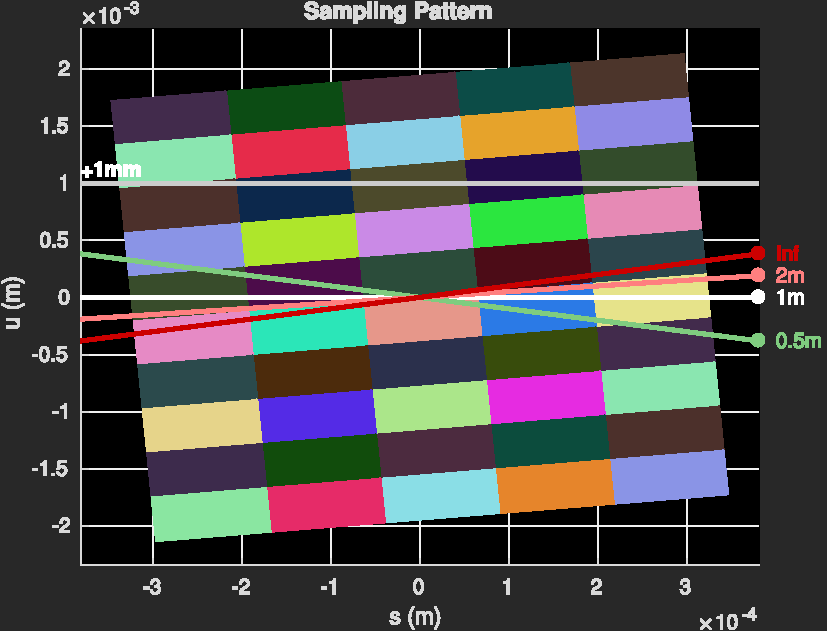
\includegraphics[width=0.48\textwidth]{Figs/STPlanePos_Plen1_NoTrack}}\hfil
	\subfloat[]{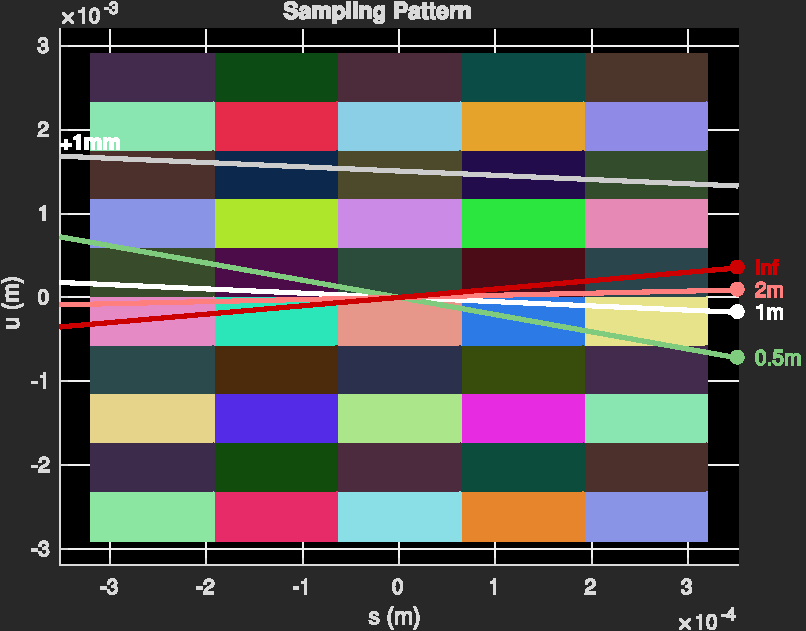
\includegraphics[width=0.48\textwidth]{Figs/STPlanePos_Plen1_Track}}\\
	\subfloat[]{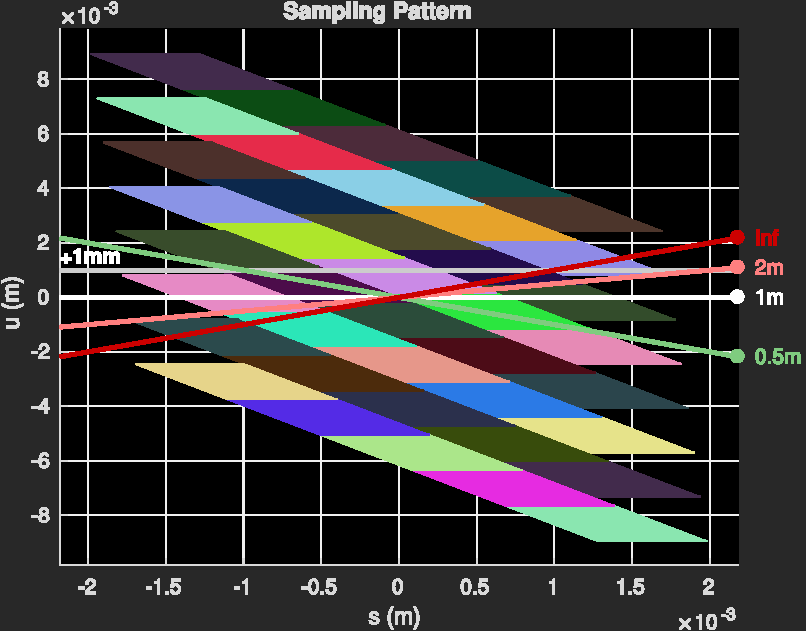
\includegraphics[width=0.48\textwidth]{Figs/STPlanePos_Plen2_NoTrack}}\hfil
	\subfloat[]{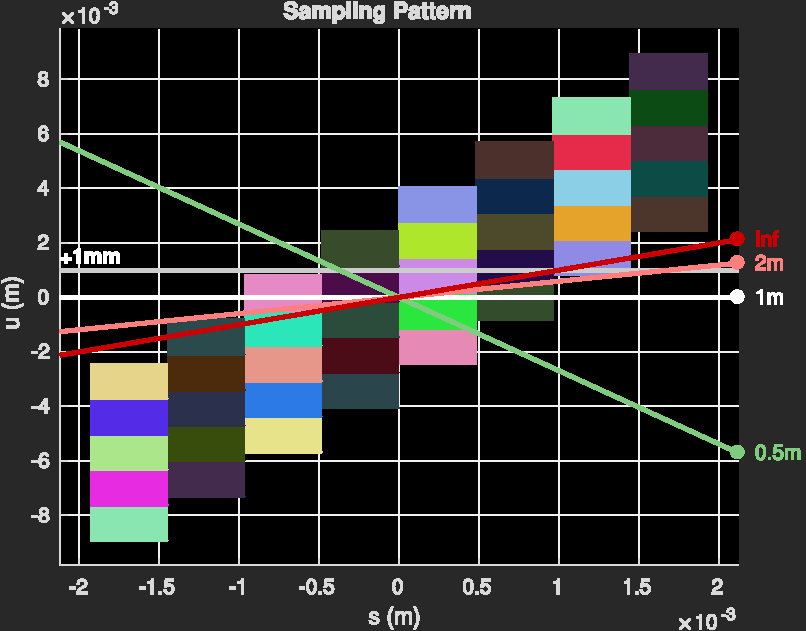
\includegraphics[width=0.48\textwidth]{Figs/STPlanePos_Plen2_Track}}
	\caption{Choice of reference plane positions for (top) a standard plenoptic camera and (bottom) a plenoptic 2.0 camera: (left) fixing the $s,t$ plane at $z=0$ and the $u,v$ plane at 1~m, compared with (right) placing the $s,t$ plane at the virtual camera array position (see main text), and the $u,v$ plane at the camera's focal depth. The two scenarios convey the same information but in different forms.}
	\label{fig_RefPlaneIntuition}
\end{figure}

As our focus is on camera design, an obvious choice is to fix the $u,v$ reference plane at a fixed depth within the scene, and the $s,t$ plane at $z=0$.  This allows direct comparison of cameras, but can yield difficult-to-understand sampling patterns, especially for plenoptic 2.0 configurations.  See, for example, Fig.~\ref{fig_RefPlaneIntuition}, for which the left images show the result of this fixed approach.  It is difficult to visually evaluate the performance of the plenoptic 2.0 camera on the bottom-left.

A few insights allow us to select reference plane locations to better build intuition. The standard plenoptic camera with $N \times N$ pixels per lenslet and $M \times M$ lenslets can be idealized as producing an $N \times N$ array of cameras floating at one focal distance in front of the main lens, with each camera having $M \times M$ pixels.

Similarly, the plenoptic 2.0 camera with the same lenslet and pixel count can be understood as producing an array of $M \times M$ cameras inside the scene, each having $N \times N$ pixels.  The position of the array depends on the focal settings of the camera, and is typically between the scene and camera, but can also be behind the scene or camera.

So both camera configurations can be thought of as virtual camera arrays.  If we fix the $s,t$ plane at this virtual camera array position, and the the $u,v$ plane at the focal depth of the camera, we can obtain better aligned sampling patterns.  This is demonstrated on the right in Fig.~\ref{fig_RefPlaneIntuition}.  Note that the depth references reflect the changes to reference plane positions, so that these figures depict the exact same information, just in a different form.

The plenoptic 2.0 example in Fig.~\ref{fig_RefPlaneIntuition} is paticularly interesting, as it is difficult to tell from the version on the left that most scene points are only seen 4 times, while this is clear by following the 1~m depth reference through the sampling pattern in the figure on the right.  It is also clear from this plot that the resolution behaviour of the plenoptic 2.0 camera is much more complex, yielding differing sample counts along $s$ based on depth.  Note that for this camera an object at infinity will be seen 6 times, while one at 0.5~m only about 2 times.

%-----------------------------
\section{The Spatial Overview Display}

\begin{figure}
	\centering
	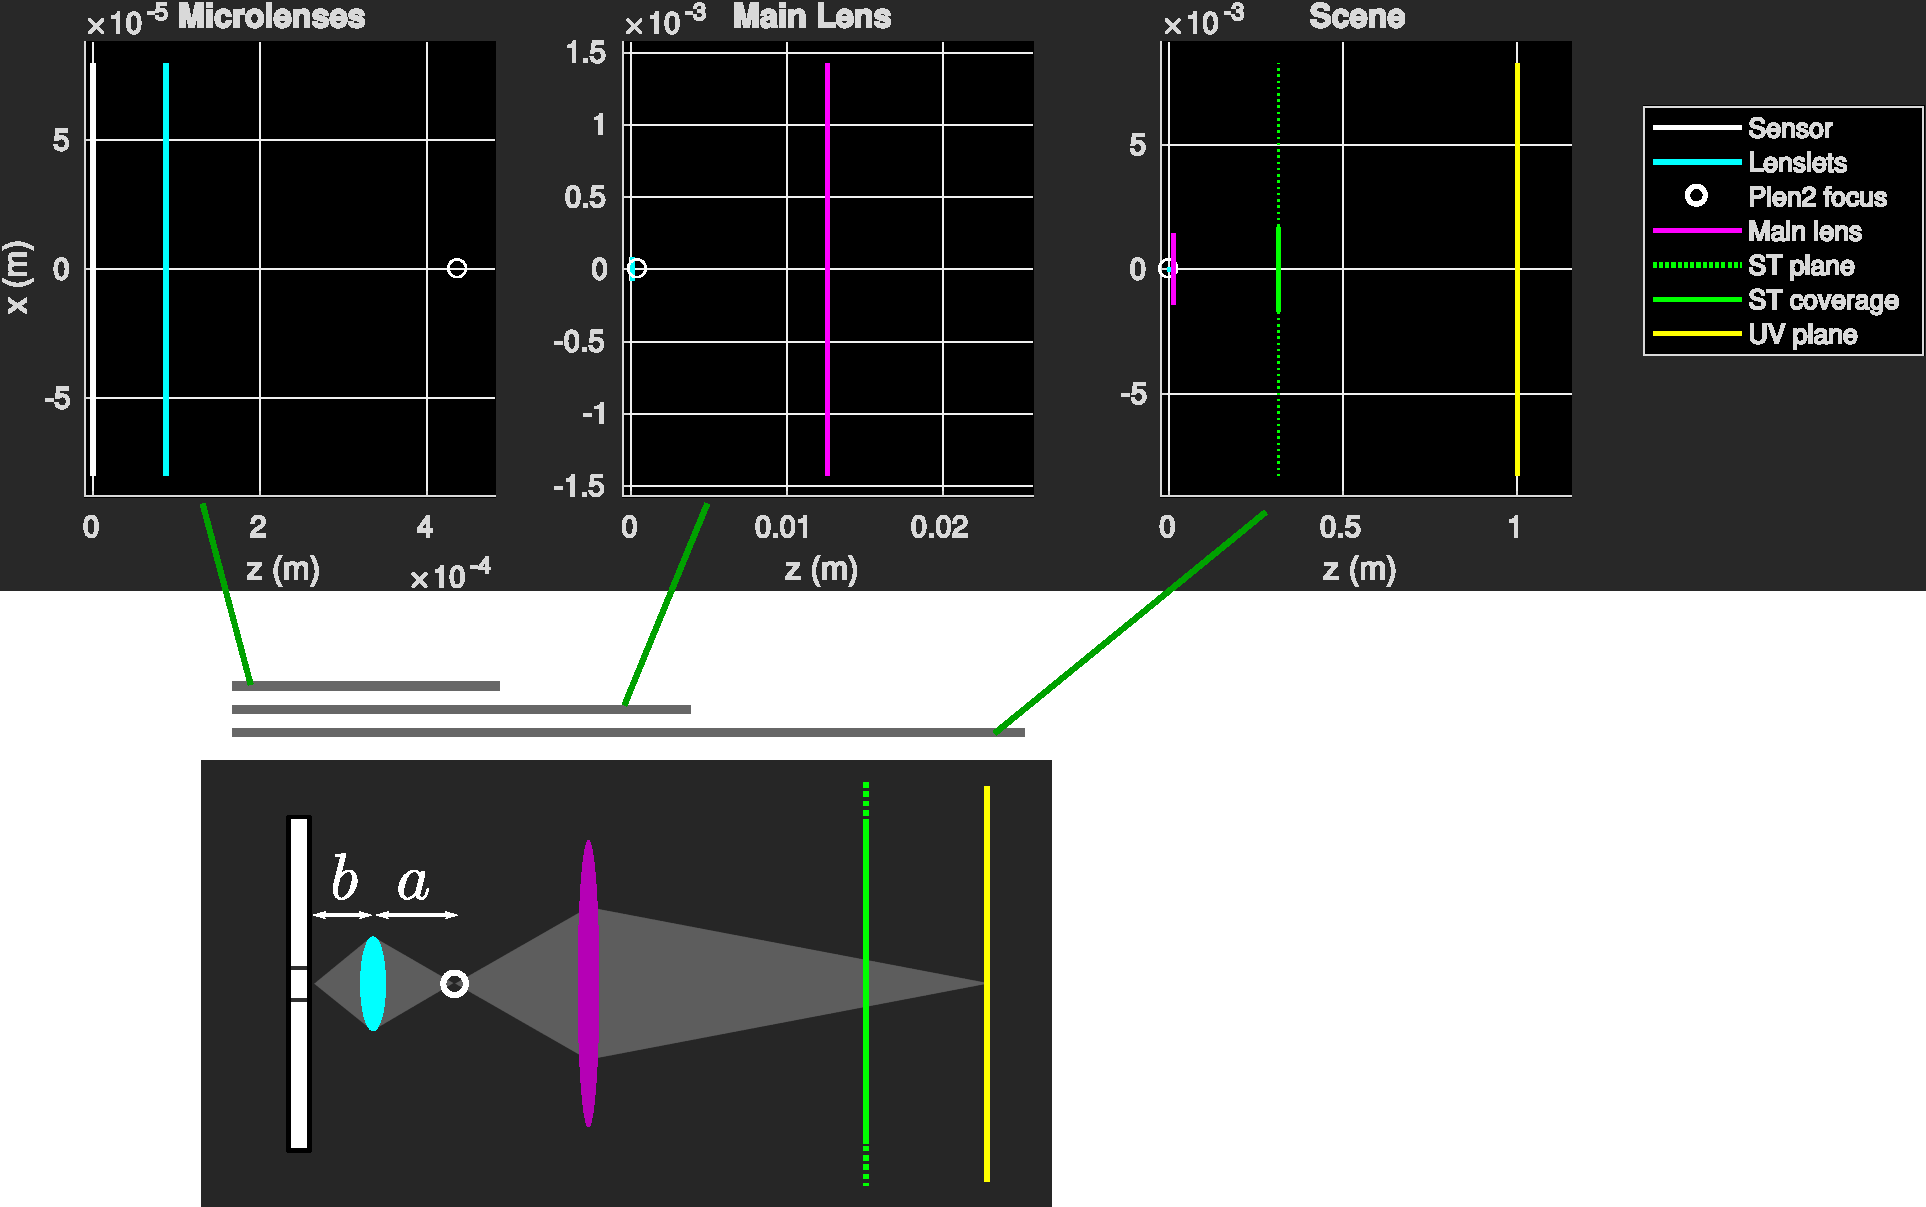
\includegraphics[width=1\textwidth]{Figs/SpatialOverview}
	\caption{The spatial overview display gives a rough depiction of the positioning between the sensor, lenslet array, main lens, reference planes and, for plenoptic 2.0 cameras, the plenoptic focal point. Depicted here are the three scales employed to convey the entire scenario.}
	\label{fig_SpatialOverview}
\end{figure}

The spatial overview depicts the physical layout of the camera, in a set of rough plots, to help build intuition and reality check a design.  Because the relevant dimensions span from micrometers to meters, this cannot be done to scale in one figure.  The spatial layout is therefore split between three figures, one at the scale of the microlenses, one at the scale of the main lens, and one at the scale of the scene.  Fig.~\ref{fig_SpatialOverview} depicts three typical figures for a plenoptic 2.0 camera, and how they relate to a not-to-scale model of a plenoptic 2.0 camera. Colour coding is maintained through the sub-plots and reference diagram, and follows the legend to the right of the figure.

%-----------------------------
\section{Explanation of Parameters}

\begin{table}
\renewcommand{\arraystretch}{1.2}
\caption{GUI-controlled display options}
\centering
\begin{tabular}{lp{24em}}
\toprule
Setting 				& Description \\
\midrule
$s,t$ plane follows...		& Controls the $s,t$ plane to the virtual camera array depth, as in Sect.~\ref{sect_RefPlaneLocations}\\
$u,v$ plane follows...		& Controls the $u,v$ plane to the focal depth, as in Sect.~\ref{sect_RefPlaneLocations}\\
$s,t$ and $u,v$ plane positions	& Manual control of the reference plane positions\\
Depth refs				& Enable and control the key depth of the depth references. Displayed are the key depth times 0.5, 1, 2 and infinity\\
$s,u$ axes autoscale	& Enable to have the epipolar plot resize to fit the sampling pattern\\
\bottomrule
\end{tabular}
\label{tab_DisplayOptions}
\end{table}

\begin{table}
\renewcommand{\arraystretch}{1.2}
\caption{GUI-controlled camera parameters}
\centering
\begin{tabular}{lp{24em}}
\toprule
Setting 				& Description \\
\midrule
Camera model			& Selects a plenoptic 1.0 or 2.0 configuration\\
Focal depth (m)			& Depth at which the camera's main lens is focused\\
Plen2 ratio				& Ratio of the focal distances $a/b$, see Fig.~\ref{fig_SpatialOverview}; only for plenoptic 2.0 cameras; negative means focus behind the lenslet array \\
Lenslet diam (pix)		& Size of a single lenslet as an integer number of pixels\\
Main focal (mm)			& Focal length of the main lens\\
Lenslet focal (\si{\micro}m) & Focal length of the microlenses\\
Pixel count				& Number of pixels to simulate\\
Pixel size (\si{\micro}m)	& Size of a single pixel\\
\bottomrule
\end{tabular}
\label{tab_CamParams}
\end{table}


\begin{table}
\renewcommand{\arraystretch}{1.2}
\caption{Computed camera parameters}
\centering
\begin{tabular}{lp{24em}}
\toprule
Setting 				& Description \\
\midrule
SensorSize (m)		& Total extent of the sensor\\
LensletDiam (m)		& Diameter of a single lenslet, in meters\\
NLenslets 			& Total lenslet count\\
MainLensDiam (m)	& Diameter of the main lens\\
MainLensDist (m)	& Position of the main lens relative to the sensor\\
LensletDist (m)		& Position of the microlens array relative to the sensor\\
Plen2FocDist (m)	& Distance of the plenoptic 2.0 focal point relative to the sensor\\
\bottomrule
\end{tabular}
\label{tab_CamParams_Computed}
\end{table}

\begin{table}
\renewcommand{\arraystretch}{1.2}
\caption{Computed performance estimate}
\centering
\begin{tabular}{lp{22em}}
\toprule
Setting 				& Description \\
\midrule
Theoretic FOV (deg)	& Field of view; typically the tool would be used with a subset of the total pixel count, but if set to the full horizontal pixel count this will reflect the camera's FOV\\
FOV Footprint (mm)	& Footprint (captured area) of the image at the focal depth, see pixel count comment above\\
Naive spatial samps & Number of samples in the $u$ direction at the focal depth, i.e.~``spatial'' samples, with respect to the scene\\
PixelFootprint  (mm) & Footprint (integrated area) for a pixel at the focal depth\\
MaxLensletAlignError (m)	& Maximum alignment error between the lenslet array and sensor planes before a pixel-sized shift is observed; this is also reported in deg.\ and arcsec\\
EffectiveFNumber 	& A number that reflects the light gathering ability of the camera: distance from main lens to lenslet array, divided by main lens diameter\\
LensletFNumber		& F number of the lenslets\\
MainLensFNumber		& F number of the main lens\\
NumAngularSamples	& Number of samples in the $s$ direction at the focal depth, i.e.~``angular'' samples, with respect to the scene\\
NaiveNearFocalLimit (m) & Near focal limit\\
NaiveFarFocalLimit (m) & Far focal limit\\
\bottomrule
\end{tabular}
\label{tab_CamPerformanceMetrics}
\end{table}

Table~\ref{tab_CamParams} summarizes the camera design parameters controlled through the GUI.  The solver uses these values to compute the camera parameters summarized in Table~\ref{tab_CamParams_Computed}.  The computed parameters currently appear in the MATLAB console, and some of them are depicted in the spatial overview figure.

A set of camera performance metrics are also estimated, and these appear in the MATLAB console. These are summarized in Table~\ref{tab_CamPerformanceMetrics}.  Use these with caution, they are experimental and can be misleading, e.g.~the number of angular samples does not map trivialy to depth resolution.


%-----------------------------
\section{Future Plans}

The experimental performance estimate is the weakest feature.  It should be upgraded to include depth resolution, a spatial resolution that takes the light field super-resolution into consideration, and ideally depth-dependent spatial and angular resolution plots.

The spatial displays are very minimalist, some way of producing a nicer display without impacting the update rate would be ideal. 

It would be better not to reset the display options on load.

This document would benefit from a section exploring practical examples.


%-----------------------------
\section{Further Reading}
\label{sect_FurtherReading}

The light field parameterization was introduced in~\cite{levoy1996light} and an excellent review of the light field structure, sampling patterns in world space, and pointers to further reading are given by Ihrke et~al in~\cite{ihrke2016principles}.  

Light field basics, parameterizations and visualization are discussed in~\cite{dansereau2014Thesis} Chap.~2, pixel integrating volumes and sampling patterns in Chap.~3.2, and the point-plane correspondence in Chap.~4.3.

Plenoptic camera design, camera-space sampling patterns and epipolar images are discussed in~\cite{ng2006digital} Chaps.~2 and~3, and the focused (plenoptic 2.0) configuration is introduced in~\cite{lumsdaine2009focused}.

%-----------------------------
\newpage
\bibliographystyle{IEEEtran}
\bibliography{LFCamExplore}



\end{document}
